%%%%%%%%%%%%%%%%%%%%%%%%%%%%%%%%%%%%%%%%%%%%%%%%
\input{preamble.ltx}

% correct bad hyphenation here; separate each word by a space
\hyphenation{op-tical net-works semi-conduc-tor}

%%%%%%%%%%%%%%%%%%%%%%%%%%%%%%%%%%%%%%%%%%%%%%%%
\begin{document}

\title{BLUETOOTH and WIFI-ENABLED PANIC BUTTON for POTENTIAL RAPE VICTIMS} %ang imomodify daw yung BLUETOOTH and WIFI

\author{
	{\small
		%\renewcommand{\arraystretch}{1.3}
		\begin{tabular}{l l l}
			& \multicolumn{2}{c}{\tiny \textcolor[rgb]{0.9,0.9,0.9}{Participated in \& did the coursework [Y/N]?}} 
			\\ 
			GUEVARRA,~Alnair~M.~(11531622) & Y & 
\includegraphics[height=5ex] {A_signature} 
			\\ 
			HERNANDEZ,~Roy~Stephen~A.~(11530731)     & Y & %\includegraphics[height=5ex]{JDC_signature}
			\\ 
			LAGMAN,~Maria~Josefa~M.~(11524855)  & Y & 
\includegraphics[height=5ex]{mama_signature} 
			\\
			MOLINA,~Adam~M.(11524855)  & Y & %\includegraphics[height=5ex]{Capture1}
			\\  		
		\end{tabular}
	}
% for author names; note positions of commas and nonbreaking spaces ( ~ ) LaTeX will not break a structure at a ~ so this keeps an author's name from being broken across two lines.
\thanks{\CrmD\protect\\} %<--Do not delete this \thanks{\CrmD\protect\\} 
 \thanks{Coursework Starting Date: \hspace{1ex} July 13, 2018}
\thanks{Submission Date: \hspace{1ex} August 18, 2018}} 

\markboth{\makebox[\columnwidth]{DIGCOMM Project \hfill}%
\hspace{\columnsep}\makebox[\columnwidth]{\hfill}}%
{} % header

\IEEEpubid{\makebox[\columnwidth]{DIGCOMM - EK \hfill DLSU}%
\hspace{\columnsep}\makebox[\columnwidth]{ \hfill {\tiny\textcolor[rgb]{0.4,0.4,0.4}{\prsDy}}}} % footer

\maketitle % for making the title area


\section{Conspectus}
\label{sec:cnspcts}

\IEEEpubidadjcol % needed in second column of first page if using \IEEEpubid

\subsection{What are the objectives of the coursework?}

\subsubsection{To assess any Digital Communications Technology (DCT) to be used in marginalized sector.}
\subsubsection{To modify the DCT appropriate to the selected marginalized sector.}
\subsubsection{To appraise the economic, societal, and environmental implications of the modified DCT.}

\subsection{How does the coursework fit with the course and previously done coursework?}
\subsubsection{This project focuses on notifying the app users immediately when panic button is pressed.}
\subsubsection{It involves the creation of a communication platform between caregivers and the elderly in case of emergencies.}

\subsection{How were the objectives achieved?}
\subsubsection{The target marginalized sector of our DCT is the elderly}
\subsubsection{Additional mode of addressing an emergency (via app) will be implemented instead of just having a buzzer when a panic button is pressed} 
%For now eto yung nilagay namin ayusin nlng natin
	


\section{Concepts and Principles}
\label{sec:concps}

\subsection{What are the necessary and relevant concepts and principles for understanding the coursework and for supporting the correct results?}
Some concepts and principles involved for understanding the coursework and for supporting the correct results includes a good understanding of android application development and proper hardware input detection with bluetooth devices.

\subsection{How does any new component, not covered in  previous coursework, function?}
Added function of online emergency notification to linked personal devices and automatic emergency hotline dialling on panic-button press.

\subsection{Did you cite more than two publications in your answers in Sec. 2.1. and 2.2}
No.
	
\subsection{Did you cite any online source in your answers in Sec.2.1 and Sec.2.2?}
No.


\section{Methodology}

\subsection{How does your implementation in Sec.~\ref{sec:implem} achieve the objectives?}
The implementation achieved the objectives by manipulating the codes used in MATLAB.
	
\subsection{Why does your implementation in Sec.~\ref{sec:implem} achieve the objectives?}
The implementation was followed accordingly that is why it achieved the objectives.
	
\subsection{How does your evaluation in Sec.~\ref{sec:eval} achieve the objectives?}
The evaluation corrected mistakes done in the project.
	
\subsection{Why does your evaluation in Sec.~\ref{sec:eval}  achieve the objectives?}
It is because the evaluation is an excellent method for assessing the codes in MATLAB  to achieve the objectives.




\subsection{Implementation}
\label{sec:implem}




\subsubsection{What were the materials used?}
The material used for the project is a laptop which contained the software MATLAB that was used to complete the project



\subsubsection{What is the summary of the processes used to make the coursework?}
The coursework was completed by using a software called MATLAB, which enables the user to manipulate matrices, plot functions, and create 3D figures by inputting their specific codes in the program. 
The researchers used MATLAB to their advantage in order to create the graphical representation of the 3D shaped bowl that is needed for the project.


\subsection{Evaluation}
\label{sec:eval}

\subsubsection{What were your procedures for evaluating the correct outcome of your coursework?}
A lot of debugging was executed in MATLAB to see whether the program works correctly or not. Researching about the unique functions of MATLAB was also done to make sure that everything inputted in the software is running correctly.
	
\subsubsection{What quantities were gathered and how have you obtained them for testing the veracity of your results?}

Some codes that were used in the project were taken from MATLAB tutorials found on the internet. These codes were tested and modified to check if it works properly and according to plan.


\section{Results and Discussions}

\subsection{How do the results achieve the objectives?}
The results achieved the objectives because the data has matched the criteria of the objectives. Visually, one can confirm that the output produces what is mentioned in the objectives.
\subsection{Why do the results achieve the objectives?}
The objectives have been met by the researchers using applications of vector analysis, therefore the results have achieved them.
	
\subsection{Are all your results correct  in accordance to what you described in Sec.~\ref{sec:eval} evaluation process? Why?} 
The researchers can confirm that all the results are correct, since the data has totally complied with the requirements of the program. The researchers were able to produce what was needed.
\subsection{What is result of the project, what does it mean if it is correct, and how does it contribute in reaching the objectives?}
The first figure here shows how the program calculates the shortest path between two points

This figure presents the computed volume inside the 3D bowl using the generation of a hundred random points.

Finally, this was the source code used for the program to work


\subsection{Did you cite more than two publications in your answers above (yes/no)?}
Yes.	


\section{Conclusions}
\label{sec:conc}

\subsection{What are the main points that should be known, remembered, and learned about the coursework?}
As potential engineers of the country, it is important for us to be able to identify and make use of vectors in different types of engineering applications. Considering that the applications of Algebra, Geometry, and vector analysis are highly significant and relevant in electronics engineering, discussions concerning this project should be considered.


\subsection{What is the gist of the inferences drawn from your results?}
Generally, the researchers recognized a pattern in identifying the useful equations and discussions when determining how to display the required output. The researchers had to make use of applications of various types of mathematics in order to merge the learnings and make inferences. It was also important for the researchers to be creative and dynamic when brainstorming for relevant key equations to produce the right output.


\subsection{Briefly, what are your comments on (1)~your results, and  (2)~future coursework if any?}
The researchers feel that the trial-and-error phases when they were coming up with the data was a very significant step for anyone that aspired to master vector analysis. The results achieved were a product of multiple attempts to encode the right commands and information. With regards to future coursework, as they have grown much more knowledgeable in real world applications of vector analysis and analytical mathematics, the researchers can predict that their capabilities and skills in vector analysis will permit them to provide better and more accurate responses to tasks concerning the field.


\bibliographystyle{IEEEtr}
\section{References} %hindi po ganto magreferences use \cite and jabref stuff
[1] Gibbs, J. (1901). \textit{Vector Analysis}.

[2] Hunt, B. (1995). \textit{A Guide to MATLAB for Beginners and Experienced Users.} Cambridge.


[4] Willis, K.F. (1934). \textit{Solid Mensuration}. London: John Wiley and Sons

\newpage
\begin{figure*}[!t]
	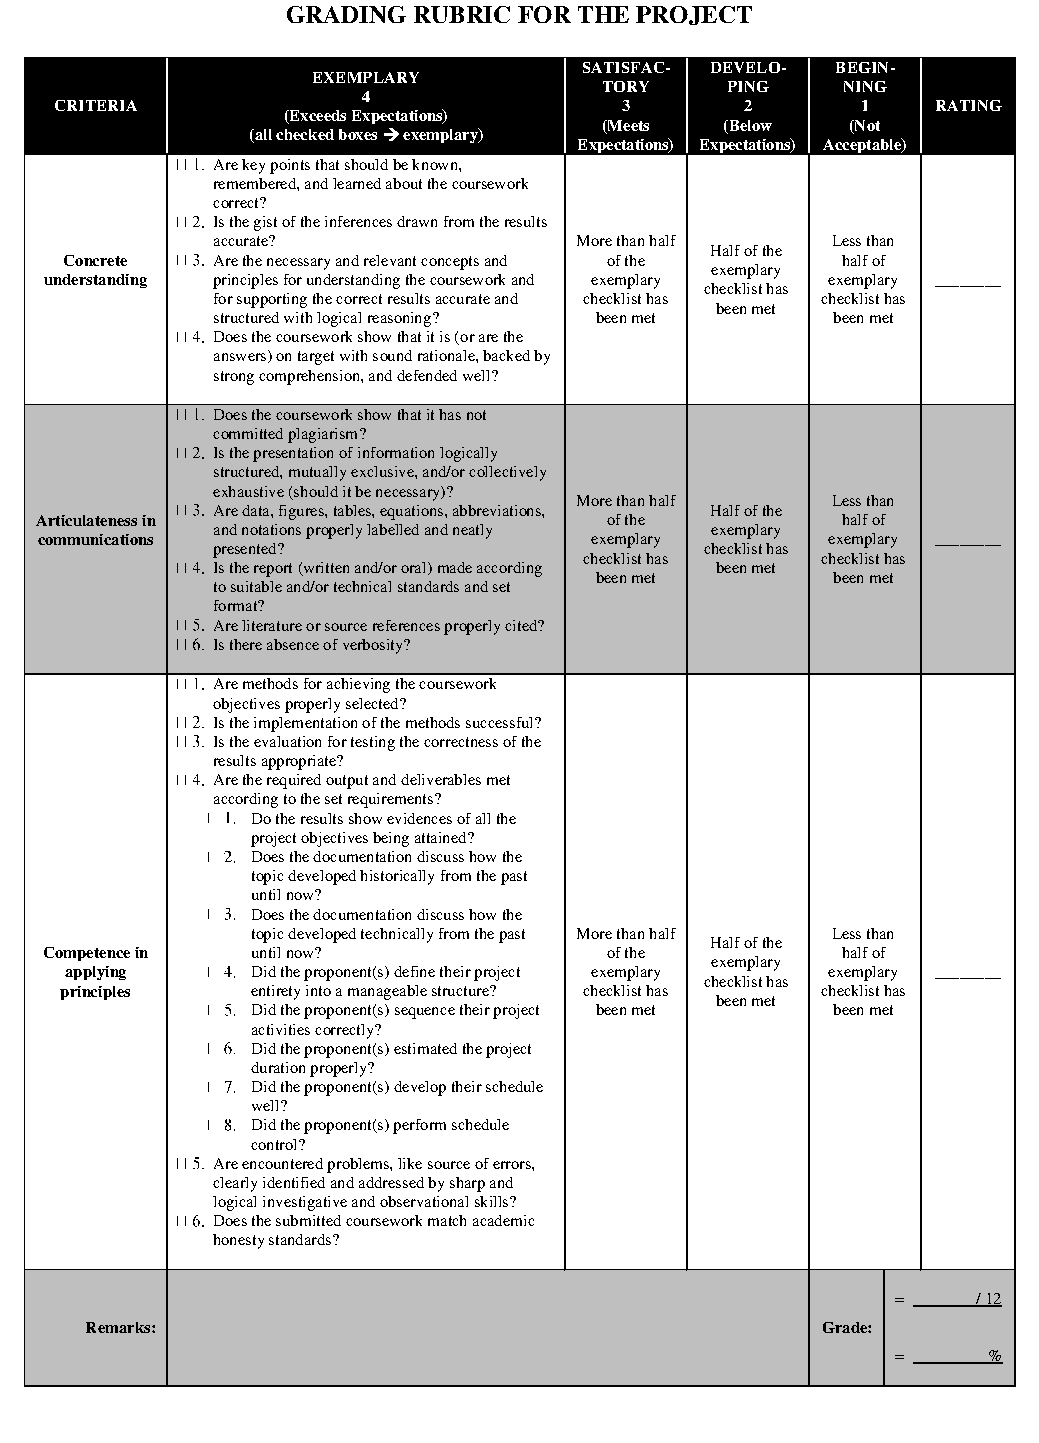
\includegraphics[width=\textwidth]{rubric} 
\end{figure*}
\cleardoublepage

\end{document}